%--------------------------------------------------------------
% moneyLaundering.tex (use thesis.tex as main file)
%--------------------------------------------------------------
\chapter{Background}
\section{Financial Crime and Money Laundering}
\label{moneyLaundering}
%--------------------------------------------------------------
Understanding how money laundering works is fundamental to garantee both an effective and explainable detection of suspicious transaction. 
This section offers a theoretical introduction to money laundering providing a mathematical formulation of the problem together with a summary of common strategies employed by criminals to avoid detection.
\subsection{The Limitations of the Lonely Scammer}
Individual scammers typically rely on simple and intuitive techniques to introduce illicit funds into the legitimate economy. One of the most prevalent methods is known as ``smurfing''. In simple terms, smurfing involves breaking down a large sum of illicit money into many smaller, inconspicuous chunks to deposit them without raising suspicion. 

More formally, individual scammers rely on smurfing to avoid Anti-Money Laundering (AML) detection mechanisms, which usually flag transactions above a specific threshold $\tilde{x}$. By splitting their initial illicit funds $x$ into smaller transactions $x_n$, such that each transaction satisfies $x_n \leq \tilde{x}$, they minimize the risk of detection \cite{contreras2026strategic}. The mathematical expectation of profit $\pi_s$ for a scammer engaging in smurfing can be defined as:
\begin{equation}
    \pi_s = x(1-\nu)
\end{equation}
where $x$ represents the total initial illicit funds, and $\nu \in (0,1)$ is the friction cost or commission proportion associated with the smurfing process (e.g., the fee paid to mules). 

While smurfing is effective for small amounts, its scalability is severely limited. When attempting to launder much larger volumes of funds, an individual scammer operating from a single account faces a significantly higher probability of detection $(1-p)$, where $p$ is the probability of successfully avoiding detection. If caught, the scammer is subjected to a severe monetary penalty $T$, which includes both the total confiscation of the funds and associated judicial fines \cite{contreras2026strategic}. Therefore, operating as a ``lonely scammer'' becomes mathematically and practically unviable for large-scale operations due to the massive expected cost of $(1-p)T$.

\subsection{Fraud Rings}
In regard to overcome those issues, criminals have improved their techniques by employing highly sophisticated obfuscation tactics. Instead of acting alone, they form complex ``fraud rings'' to distribute illicit funds across vast networks of temporary accounts. To further break the traceable link between sender and receiver, illicit actors frequently use cyclic transfers and cryptocurrency \textbf{mixers} services that pool together funds from multiple users, mix them, and redistribute them at random intervals and amounts. These advanced tactics create dense, highly camouflaged transaction topologies that easily evade threshold-based rules and simple heuristic detection methods.

To achive their goal they utilize a strategy of transaction layering, often characterized by a topological depth $L$, and network diversification to obscure the money trail \cite{contreras2026strategic, li2025scamsweeper}.
By spreading the funds through a complex topology, the fraud ring successfully increases its non-detection probability $p_L$, which now depends explicitly on the layering depth $L$. The expected profit of a fraud ring utilizing $L$ layers can be mathematically expressed as:
\begin{equation}
    E[\pi_L] = p_L x - (1-p_L)T - c(L)
\end{equation}
where $E[\pi_L]$ is the expected profit, $p_L$ is the enhanced probability of evading detection when $L$ layers are used, $x$ is the total illicit funds, $T$ is the total penalty if caught, and $c(L)$ represents the monotonic cost function associated with establishing and maintaining the $L$ transaction layers. Because the fraud ring dramatically increases the probability of evading detection ($p_L \to 1$ as $L$ increases), the expected payoff remains highly profitable even when factoring in the complex layering costs $c(L)$ \cite{contreras2026strategic}. 

\subsection{Money Laundering patterns}\label{mlpatterns}
Understanding the structural patterns that criminality assumes is fundamental to develop effective detection models and to employ strategies to enhance the explainability of them. According to the literature, there are 8 different patterns that are often used in ML \cite{AMLSim, AMLWorld}. 
\begin{figure}
    \centering
    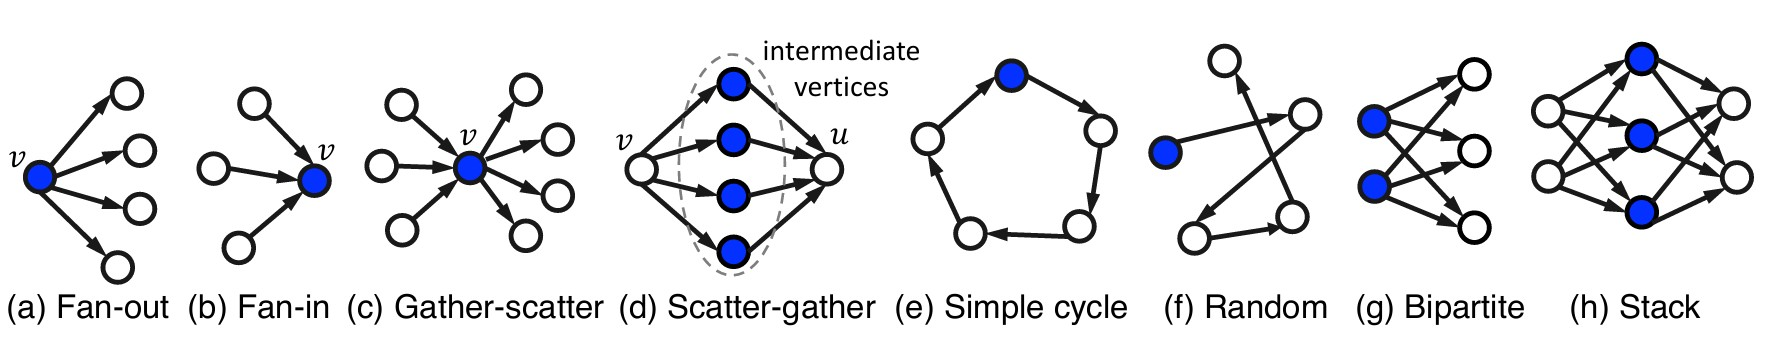
\includegraphics[width=1\textwidth]{IMG/laundering_patterns.jpg}
    \caption{Money Laundering patterns}
    \label{fig:launderingPatterns}
\end{figure}
Which are: 
\begin{itemize}
    \item \textit{fan-out}, shown in Figure \ref{fig:launderingPatterns} a, characterized by outgoing edges from a node $v$ to more than 2 adjacent nodes; 
    \item \textit{fan-in}, Figure \ref{fig:launderingPatterns} b, $v$ is connected to more than 2 nodes by incoming edges;
    \item \textit{gather-scatter}, Figure \ref{fig:launderingPatterns} c, is the combination of a fan-in and a fan-out pattern on the same node $v$;
    \item \textit{scatter-gather}, Figure \ref{fig:launderingPatterns} d, also composed by a fan-in and a fan-out pattern but on two different nodes, sharing the same intermediate neighbors;
    \item \textit{simple-cycle}, Figure \ref{fig:launderingPatterns} e, characterized by a sequence of transactions that starts and ends at the same node;
    \item \textit{random}, Figure \ref{fig:launderingPatterns} f, similar to the cycle but founds do not return to the original account;
    \item \textit{bipartite}, Figure \ref{fig:launderingPatterns} g, moves founds from a set of original nodes to a set of target nodes, with no transactions between accounts of the same set;
    \item \textit{stack}, Figure \ref{fig:launderingPatterns} h, extends the bipartite pattern by adding a second bipartite layer.
\end{itemize}
It's important to mention that in some cases some patterns can be found in both illicit and licit transactions \cite{AMLgentex}. Specifically, \textit{fan-in} and \textit{fan-out} are patterns that are also frequent in legitimate, every-day transactions, such as salary payments or transfers between family members or friends.
That being said, the detection of such patterns remains a foundamental component of any money laundering detection models, albeit insufficient on its own.
Furthermore, a model that correctly classifies those patterns provides a much more interpretable result than one that simply performs a binary classification between licit and illicit transactions. In Section \ref{ethics_privacy_regulations} we will see why explainability is of fundamental importance in the financial field. 

\section{Ethics, Privacy and Regulations}
\label{ethics_privacy_regulations}
In this section we will begin by introducing a brief overview of the regulations that currently govern the field of AML.
Subsequently a discussion on the main issues that the use of ML models may introduce will be provided, toghether with suggested solutions to address them. A special focus will be reserved to the issues of explainability and privacy.
To conclude we will consider the use of Synthetic Datasets as a possible solution to these issues, analyzing their limits and advantages in the context of AML.
\subsection{AML Global Regulations}
Effective ML detection requires a combination of domestic laws, regulatory oversight, and international cooperation. Since the end of the 20th century the United States and the Eureopean Union as key jurisdictions, toghether with the FAFT \footnote{The Financial Action Task Force (FATF) is an intergovernmental policymaking body established in 1989 by the G7} as the global leading standard-setter have been developing and elaborate framework for AML \cite{regulations}.

In 1989 the G-7 nations enstabished an inter-governmental task force to develop and promote international guidelines in regard to fight money laundering, the FATF. Nowadays FAFT still holds a central role in the AML field. It has issued 40 recomendations for national laws and international cooperation \cite{regulations}.
These principles have been adopted by over than 200 jurisdictions and they fall into 5 main areas \cite{ruleBased}:
\begin{itemize}
    \item Risk Based Approach (RBA): jurisdictions must identify and understand the financial crime risks that they face, allocating the right amount of resources to mitigate them;
    \item Legal Framework: members nations must adopt laws that criminalize money laundering; furthermore authorithies must be given the power to freeze and confiscate funds when needed;
    \item Preventive Measures:
    \begin{itemize}
        \item Customer Due Diligence (CDD): financial instututions must verify the identity of their customers;
        \item Ultimate Beneficial Ownership (OBO): company's owners must be verified, this adresses the issue of criminals hiding behind shell instututions;
        \item Record Keeping: financial instututions must mantain their transactions recrds for at least 5 years and file Suspicious Transactions Reports (STRs) to Financial Intelligence Units (FIUs).
    \end{itemize} 
    \item Supervision and Transparency: regulators must actively supervise financial instututions; members nations must immediatly enforce UN financial sanctions when required to.
    \item International cooperation: members must quickly share information and provide mutual legal assistance in international investigations.
\end{itemize}
In regard to those guidelines FAFT keeps a \textit{black-list} and a \textit{grey-list} of jurisdictions that are not compliant with its standards \cite{regulations}.

\subsection{Ethical and practical issues} \label{patterns}
When considering real-world datasets, models that detect financial crime are trained on sensitive data that needs to be protected. To avoid the leakage of sensitive information, before feeding ML models, it is necessary to apply privacy-preserving techniques. The most common practice is to apply differential privacy, which adds noise to the dataset to protect individual data points. That noise can be quantified using the privacy budget $\epsilon$, which determines the trade-off between privacy and utility. All this comes at the cost of reducing the accuracy of the model.

Another significant issue to consider is explainability. Regulators require banks to explain their decisions, and this requirement extends to the ML models they use. Deep Learning models, albeit generally more precise and powerful than traditional ML models, are often \textit{black-boxes}, meaning their decision process is very difficoult to understand for a human being.  

Real datasets are also often limited by the fact that the informations are not shared accross jurisdictions, making it difficult to detect frauds that cross borders.

To tackle all those problematics researchers at IBM developed a simulator for generating realistic financial transactions, called AMLWorld (2023) \cite{AMLWorld}. This simulator solves the privacy problem, simulates multi-jurisdictional transactions and it even tries to takle the explainability issue by providing as lable not only a boolean value for the presence of a fraud, but also the ML pattern that caracterized it. This wouldn't be possible in real life, but models trained on this synthetic dataset could be able to generalize the detection of patterns even in real world scenarios, highly enhancing interpretability.
Figure \ref{fig:amlsim_architecture} provides an overview on how AMLWorld generates realistic financial transactions and patterns of financial crime. 

The possible laundering patterns are the one described in Section \ref{mlpatterns}; the model assumes the existence of 9 different surces of criminal activities: extortion, loan sharking, gambling, prostitution, kidnapping, robbery, embezzlement, drugs, and smuggling. The amount of money and the frequency of these criminal enterprises vary by both activity category and acting entity \cite{AMLWorld}. The funds are then inserted in the financial system alongside the legit ones.
\begin{figure}
    \centering
    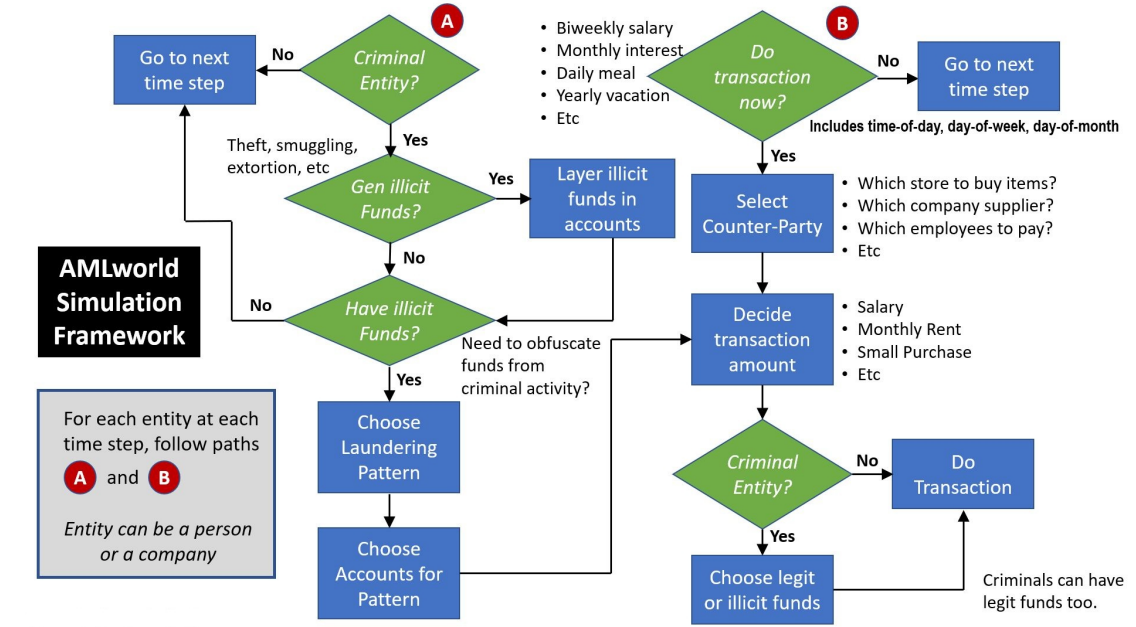
\includegraphics[width=1\textwidth]{IMG/AMLWorld.png}
    \caption{Overview of AMLworld simulation \cite{AMLWorld}}
    \label{fig:amlsim_architecture}
\end{figure}

\section{Task}
\label{task}
In this dissertation we consider the problem of Edge-Level ML detection. This means, considering the Graph $G = (V, E)$ as in Definition \ref{financialGraph}, trying to learn a function \(f\) that, for each transaction $e \in E$, predicts its class. In particular we will consider two different settings. A binary classification where each edge is labeled as fraudulent or lecit and a multi-class classification where, in case of illicit transaction, we also predict the type of pattern, amongst the one described in Section \ref{mlpatterns}, it's involved in.

Formally we seek a function \(f\) that minimizes the error \(L(f)\) over a distribution \(\mathcal{D}\) of Graphs.
\begin{equation}
    \operatorname{argmin}_{f \in \mathcal{H}} \left\{L(f) \doteq \mathbb{E}_{(x,y) \sim \mathcal{D}} [l(f(x), y)]\right\}
\end{equation}
Practically there's no way to know \(\mathcal{D}\). Instead we will consider a dataset \(G_D = (V_D, E_D)\), where both nodes and edges are equipped with feature vectors and we will seek a function \(f\) that minimizes \(L(f)\) over this dataset computing the empirical risk:
\begin{equation}
    \operatorname{argmin}_{f \in \mathcal{H}} \left\{\hat{L}(f) \doteq \frac{1}{|E_D|} \sum_{e \in E_D} l(f(x_e), y_e)\right\}
\end{equation}
This is just the theoretical overview of the problem. In Chapter \ref{approaches} we will provide more insights on how to define the hypothesis space \(\mathcal{H}\) and the loss function \(l\). 

As mentioned in Section \ref{ethics_privacy_regulations}, the strict privacy regulations that governs the financial world, makes it hard to find real-world datasets. In this dissertation, for the reasons explained in Section \ref{patterns}, we will use the synthetic dataset \textit{IBM AMLSim}. This is perfect for our scope, since it provides edge lables for both binary and multiclass classification.

\subsection{Dataset description}\label{sec:datdesc}
The IBM AMLSim dataset comes in 6 different versions.
\begin{itemize}
    \item HI-Small
    \item HI-Medium
    \item HI-Large  
    \item LO-Small
    \item LO-Medium
    \item LO-Large
\end{itemize}
Where HI (High) and LO (Low) indicate the frequency of illicit transactions and the suffixes Small, Medium and Large indicate the size of the dataset. Figure \ref{fig:datasetstats} shows the differences between the 6 datasets.
\begin{figure}
    \centering
    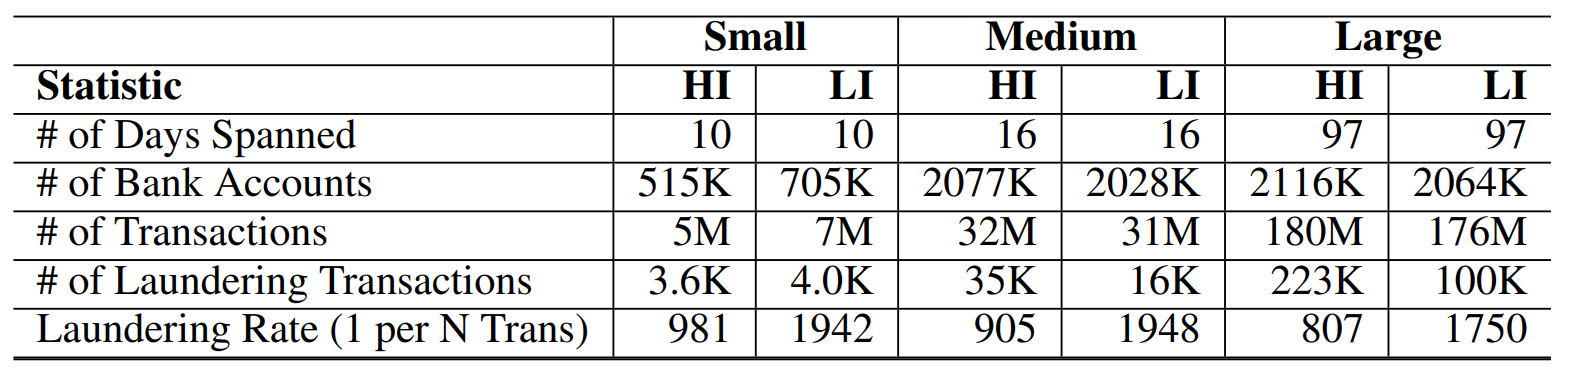
\includegraphics[width=1.0\textwidth]{IMG/dataset.png}
    \caption{IBM AMLSim datasets statistics \cite{AMLWorld}}
    \label{fig:datasetstats}
\end{figure}

In this work we will use the HI-Small version. Bigger datasets would of course garantee a better generalization and accuracy but, for hardware and time constraint, it would be impossible to train the models on such graphs. That begin said, we belive that the obtained results are good enough to understand how the models would perform in a real world scenario.

The HI-Small dataset is composed of 3 different files:
\begin{itemize}
    \item \texttt{HI-Small\_account.csv}, contains 518,581 accounts toghether with their features:
    \begin{itemize}
        \item \textit{Entity ID}: The ID of the account;
        \item \textit{Entity Name}: The name of the account;
        \item \textit{Bank Name}: The name of the bank holding the account; 
        \item \textit{Bank ID}: The ID of the bank holding the account;
        \item \textit{Account Number}: The number of the account;    
    \end{itemize}
    Figure \ref{fig:accountshead} shows some examples of account records.
    \item \texttt{HI-Small\_Trans.csv}, contains transactions features and binary labels:
    \begin{itemize}
        \item \textit{Timestamp}: The timestamp of the transaction;
        \item \textit{From Bank}: The ID of the sending bank;
        \item \textit{From Account}: The ID of the sending account;
        \item \textit{To Bank}: The ID of the receiving bank;
        \item \textit{To Account}: The ID of the receiving account;
        \item \textit{Amount Received}: The amount of money received by the recipient;
        \item \textit{Receiving Currency}: The currency of the received amount (USD, EUR, etc.);
        \item \textit{Amount Paid}: The amount of money paid by the sender;
        \item \textit{Payment Currency}: The currency of the paid amount;
        \item \textit{Payment Format}: The format/method of the payment;
        \item \textit{Is Laundering}: Binary label indicating whether the transaction is illicit;
        \item \textit{src}: Source node identifier;
        \item \textit{dst}: Destination node identifier;
    \end{itemize}
    Figure \ref{fig:transhead} shows some examples of transaction records.
    \item \texttt{HI-Small\_Patterns.txt}, lists the edges that are involved in ML activities toghether with the type of pattern they are involved in (multiclass labels).
    Examples of the 8 differt types of ML patterns in IBM AMLSim are shown in Figure \ref{fig:patternsIBM}.
\end{itemize}
\begin{figure}
    \centering
    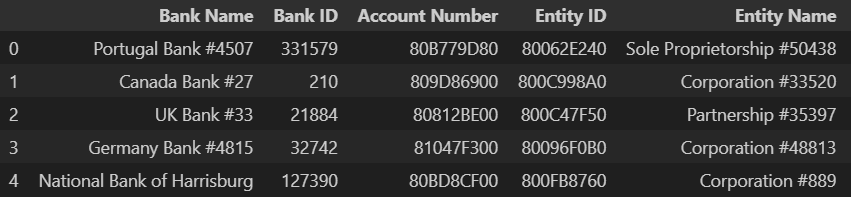
\includegraphics[width=1.0\textwidth]{IMG/accounts_head.png}
    \caption{IBM AMLSim account records}
    \label{fig:accountshead}
\end{figure}
\begin{figure}
    \centering
    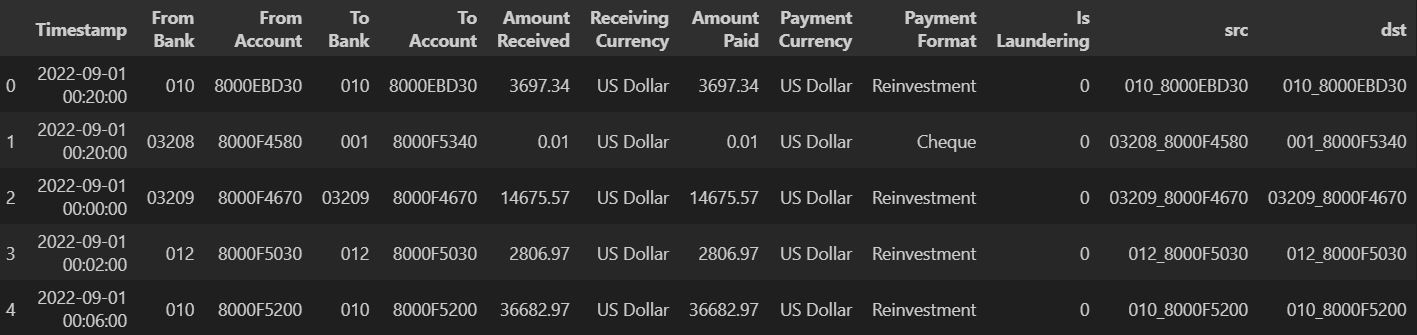
\includegraphics[width=1.0\textwidth]{IMG/trans_head.png}
    \caption{IBM AMLSim transaction records}
    \label{fig:transhead}
\end{figure}
\begin{figure}
    \centering
    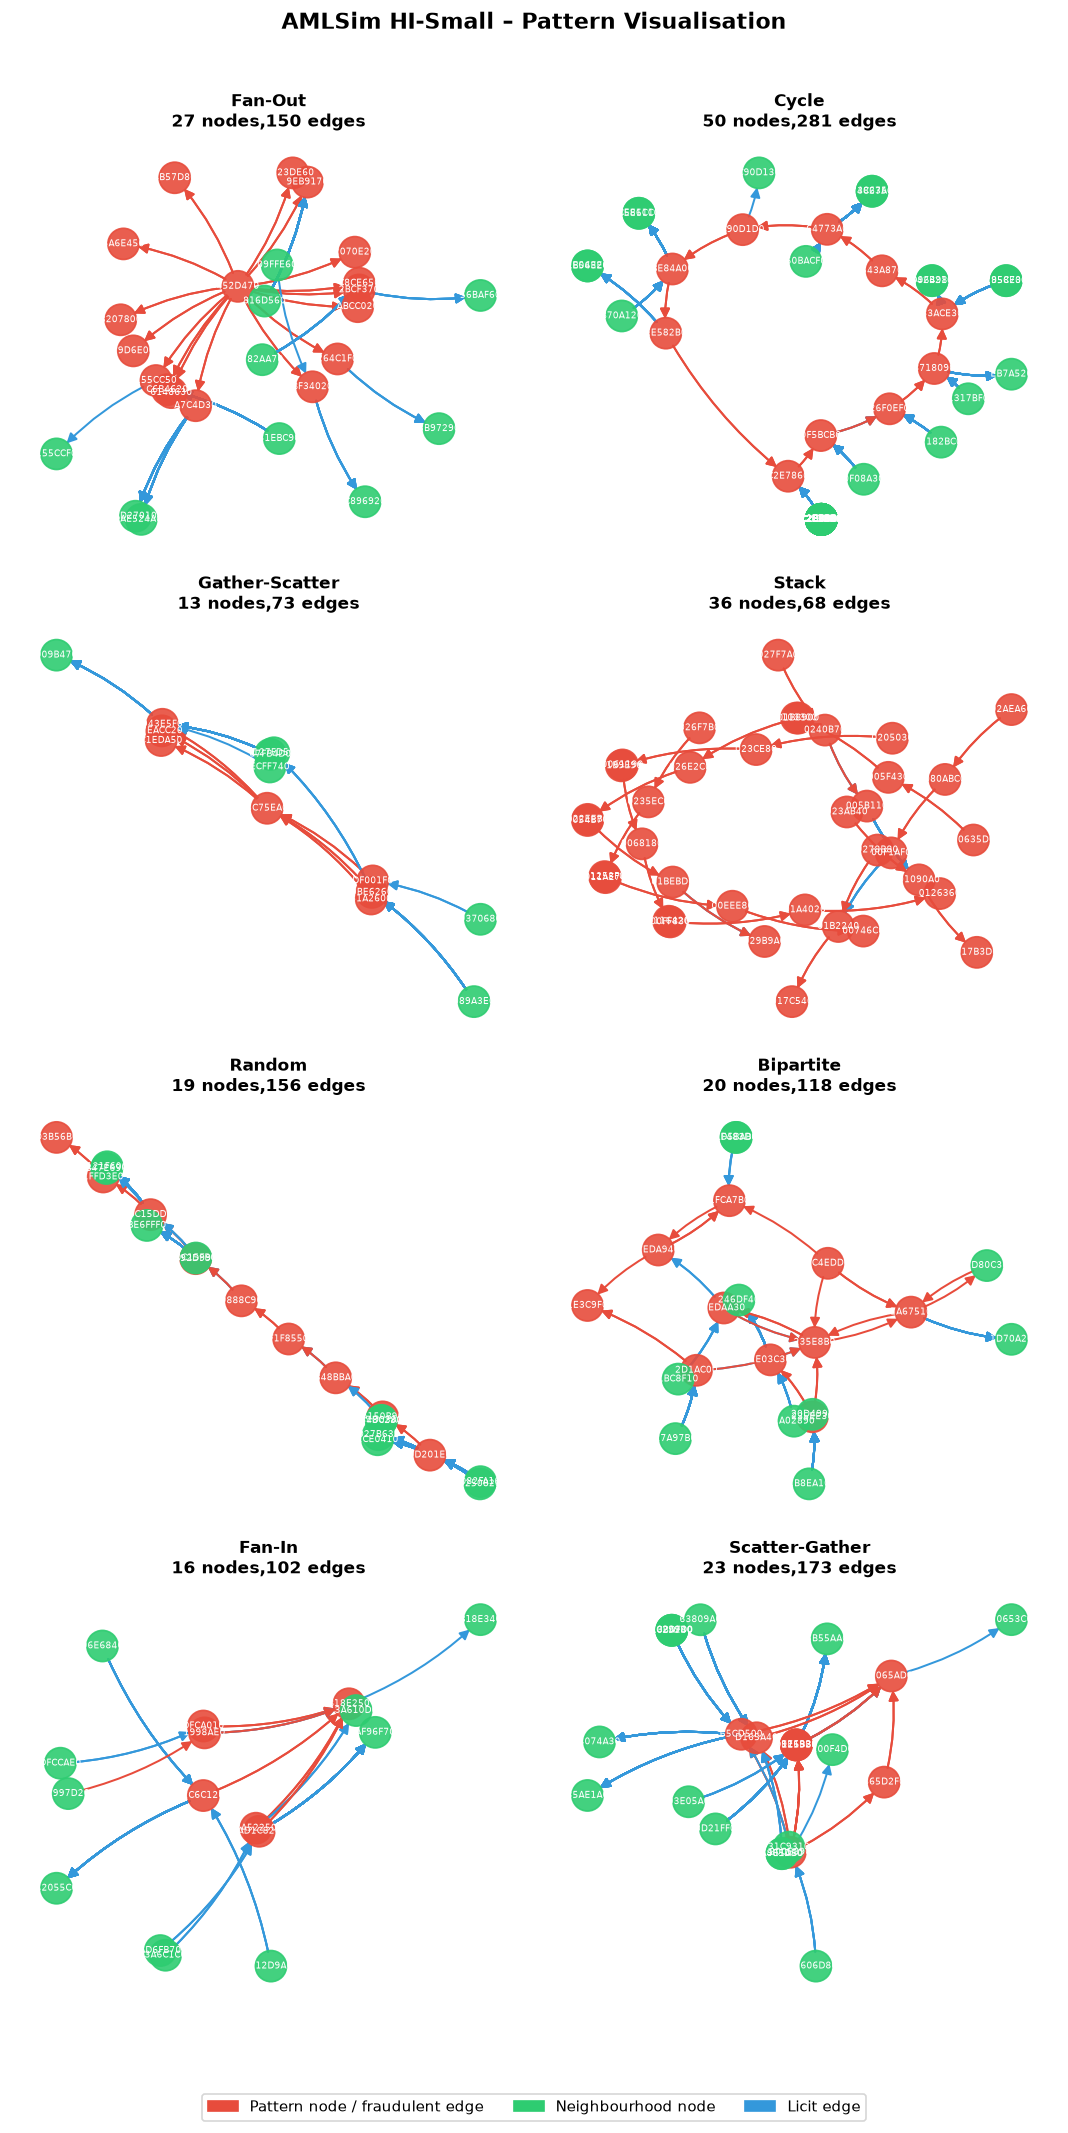
\includegraphics[width=0.76\textwidth]{IMG/patterns.png}
    \caption{IBM AMLSim patterns examples}
    \label{fig:patternsIBM}
\end{figure}
\subsection{Features analysis}
In this section we provide a detailed analysis of the edges and nodes features distributions. Before diving into that we first take a look at the distribution of the labels in the dataset. There are \(5,177\) illicit transactions over a total of \(5,078,345\) Edges.
Figure \ref{fig:patterns_distr}, provides the distribution of the multiclass label (type of pattern) over the fraudulent edges. It's important to notice that this information is provided only for \(3,149\) out of the \(5,177\) illicit transactions. This issue will be addressed in Section \ref{dataprep}.
\begin{figure}
    \centering
    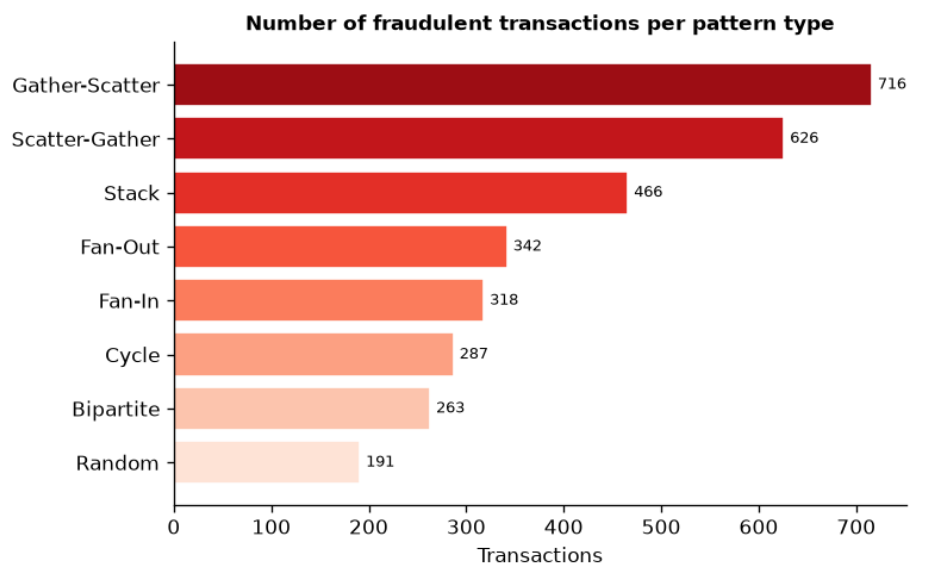
\includegraphics[width=0.8\textwidth]{IMG/patterns_distr.png}
    \caption{IBM AMLSim patterns distribution over fraudulent edges}
    \label{fig:patterns_distr}
\end{figure}

We now procede by analyzing the edge features. First, we notice that \textit{Amount Received} and \textit{Amount Paid} are almost identical. From Figure \ref{fig:amounttrans} we can see that fraudulent trasnactions have the tendency to be bigger than lecit ones.

Continuing our analysis on edge features, we notice that the most common currency is USD for both fraudulent and licit transactions; most of the currencies have a similar proportion distribution from both fraudulent and licit transactions. From Figure \ref{fig:currencytrans} we can see that there are two exceptions: Shekel, which is more prevalent in licit transactions, and Saudi Riyal, which is significantly more prevalent in fraudulent transactions. It's important to notice that the graph shows the proportion of each currency with respect to the total number of transactions in each class; Since there are way more licit than fraudulent transactions, having similar distributions means that, for every type of currency, licit transactions still represent the vast majority.

Considering now the payment formats, by looking at Figure \ref{fig:paymentformats} we notice that ACH transactions are more frequently used for fraudulent transactions compared to other methods.

The last edge feature is \textit{Timestamp}. Since working with timestamps can be tricky, we decided to extract to categorical features representing the hour of the day and the day of the week (Figures \ref{fig:hourday}). Normally we would have also considered the week of the year and the year itself but, since IBM AMLSim Small only covers the span of a week, it would be irrelevant. That being said, it's important to mention that directly working with timestamps, albeit tricky, could lead to a more precise detection [Chapter \ref{futureDirections}]. 
\begin{figure}
    \centering
    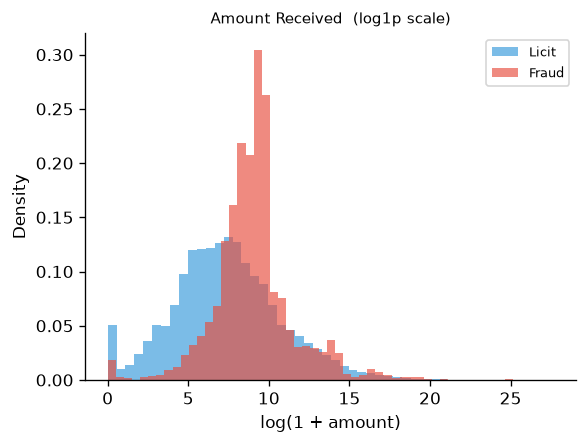
\includegraphics[width=0.8\textwidth]{IMG/amount.png}
    \caption{IBM AMLSim amounts distribution}
    \label{fig:amounttrans}
\end{figure} 
\begin{figure}
    \centering
    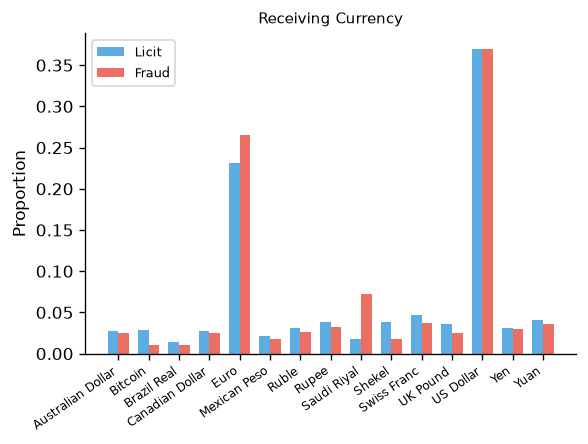
\includegraphics[width=0.8\textwidth]{IMG/currencies.png}
    \caption{IBM AMLSim currencies distribution}
    \label{fig:currencytrans}
\end{figure} 
\begin{figure}
    \centering
    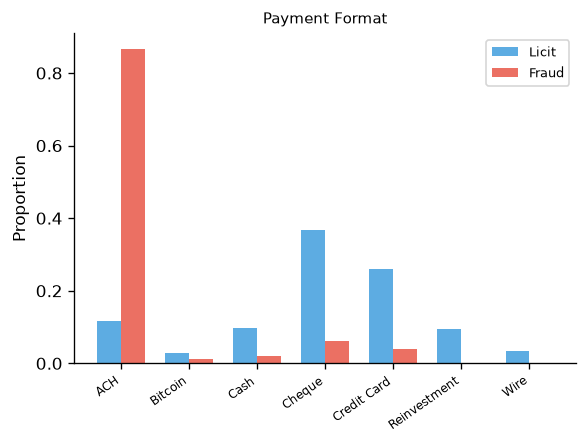
\includegraphics[width=0.8\textwidth]{IMG/format.png}
    \caption{IBM AMLSim payment formats distribution}
    \label{fig:paymentformats}
\end{figure} 
\begin{figure}
    \centering
    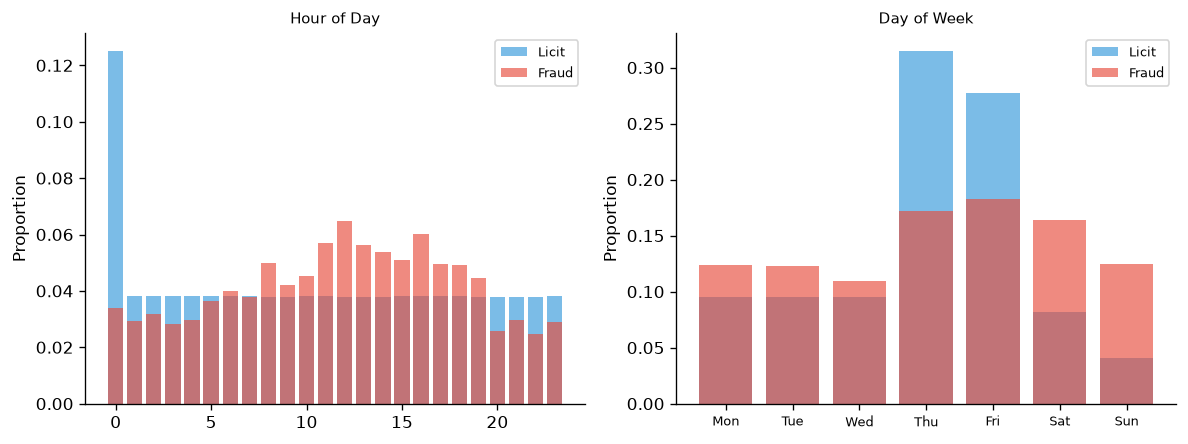
\includegraphics[width=0.8\textwidth]{IMG/hourday.png}
    \caption{IBM AMLSim hour and day of the week distributions}
    \label{fig:hourday}
\end{figure} 

Finally we take a look at the Node features. The only intresting one is \textit{Bank Name}, Figure \ref{fig:bank} shows the distribution of licit and illicit nodes over the 10 biggest banks.
\begin{figure}
    \centering
    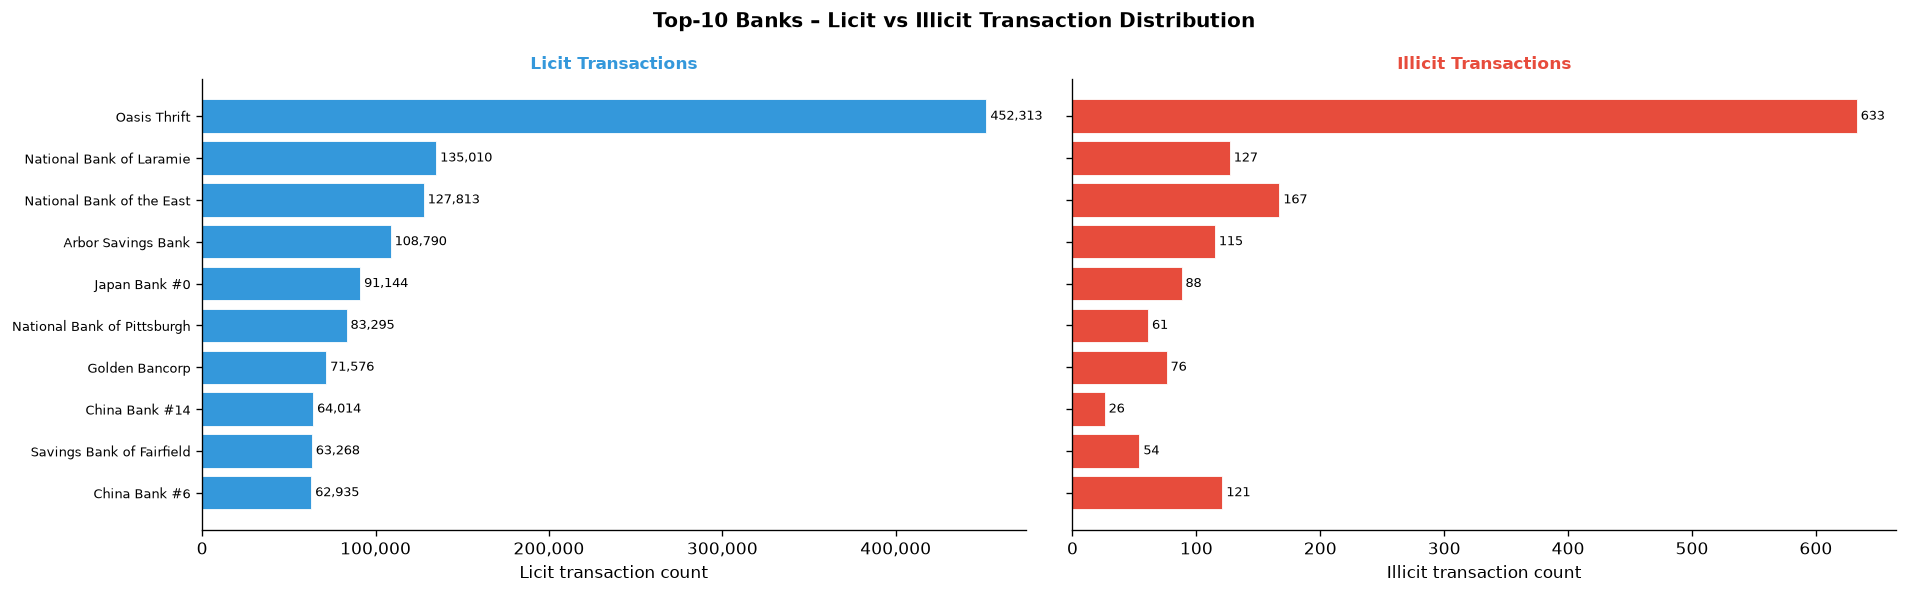
\includegraphics[width=0.8\textwidth]{IMG/banks.png}
    \caption{IBM AMLSim banks distribution}
    \label{fig:bank}
\end{figure} 